%Para figuras \begin{figure}[H] % {{{*
   % \centering
    %
\includegraphics[width=0.8\textwidth]{RectangleStateTimeEvol.pdf}
    %\caption{Evolución de un estado localizado con estado inicial de moneda $(1,1,1,1)$ en el tiempo $t=275$ pasos. Dimensiones del estadio: $L_x=200$, $L_y=175$. Moneda de Grover: $\pi/4$.}
%\end{figure} % *}}}
\documentclass[12pt,a4paper]{article} % {{{*
\usepackage[utf8]{inputenc}
\usepackage[spanish]{babel}
\usepackage{float}
\usepackage{amsmath}
\usepackage{amsfonts}
\usepackage{subcaption}
\usepackage{amssymb}
\usepackage{graphicx}
\usepackage{hyperref}
\usepackage{braket}

\usepackage{xcolor}
\usepackage[draft,inline,nomargin]{fixme} \fxsetup{theme=color}
\definecolor{jacolor}{RGB}{200,40,0}
\FXRegisterAuthor{ja}{aja}{\color{jacolor}JA}

\graphicspath{{Imgs/}}
\title{Dinámica de caminatas cuánticas\\
Con una moneda de 4D}
\author{}
\date{}

% *}}}
\begin{document}
\maketitle
\janote{Faltan resultados sobre el promedio temporal de la distribución de probabilidad (la que tiene una distribución límite)}
\janote{Lo importante aquí era que aparecían dos cosas: (1) localización en el sito inicial que es característica de la moneda de Grover (explicación en un paper de Aharonov \cite{aharonov2001quantum}, creo, Saul sabe), (2) patrones de localización siempre que la geometría es integrable, y ausencia de los patrones cuando la geometría es caótica}
\janote{Faltan resultados sobre la IPR}
\tableofcontents
\newpage
\section{Generalidades} % {{{*
El estado de un caminante pertenece al espacio de Hilbert $\mathcal{H}=\mathcal{H}_c\otimes \mathcal{H}_p $, siendo $\mathcal{H}_c$ y $\mathcal{H}_p$
espacios de Hilbert de la moneda y de la posición, respectivamente.
La evolución de un caminante viene descrita por el operador evolución $\mathcal{U}$ tal que si $\ket{\psi_0}$ es un estado inicial en el tiempo $t = 0$,
entonces:
\begin{equation}
\ket{\psi_1}=U\ket{\psi_0}.
\end{equation}
representa el primer paso del estado inicial $\ket{\psi_0}$.
Por inducción se deduce que, a un n-ésimo paso :
\begin{equation}
\ket{\psi_n}=U \ket{\psi_{n-1}}=U^{n} \ket{\psi_0}.
\end{equation}
Pues $\mathcal{U}$ es unitaria, sus eigenvalores son de norma 1 y por tanto conviene estudiar las fases de dichos valores.
A la fase asociada al eigenvalor dado se le llamará eigenfase.

La forma de definir $U$ que se seguirá en estas notas es la siguiente:
\begin{equation}
\mathcal{U}=S\cdot C.
\end{equation}
Siendo $S$ un operador que desplaza al caminante según su estado de moneda y $C$ un operador que actua sobre el estado de moneda del caminante.

Es de mencionar que la presencia de condiciones de frontera está cifrada en la estructura del operador $S$.
La dinámica resultante depende de la elección de $C$ y del tipo de condiciones de frontera a escoger.
No es claro cuales son las condiciones sobre las cuales emerge caos cuántico (elección de moneda $C$, condiciones de frontera, etc \dots)

% *}}}

\section{Acerca de la limit distribution.}
Considerando que $dim(\mathcal{H}_c)=4$ y un dominio espacial $\Omega$ tal que si $(x,y)\in \Omega$ entonces $\ket{x,y}\in \mathcal{H}_p$.
Sea $v$ el nodo asociado a la coordenada $(x,y)$, luego
$$
\ket{c_i}\otimes\ket{v}=\ket{c_i,v}.
$$
representa un estado localizado en la posición $v=(x,y)$ con estado de moneda $c_i$.
Defínase la probabilidad de hallar al caminante en la coordenada $v=(x,y)$ en un tiempo $t$ partiendo del estado inicial $\ket{\alpha_0}$, independientemente de su estado de moneda, según~\cite{aharonov2001quantum}:
\begin{equation}
    P_t(v|\alpha_0)=\sum_{k}|\braket{c_k,v|\alpha_t}|^{2}.
    \label{eq:SiteProb}
\end{equation}
Esta cantidad no converge a un límite asintótico.

Así mismo se define la distribución límite, \textit{limit distribution}~\cite{aharonov2001quantum}, la cual es el promedio temporal de \eqref{eq:SiteProb}.
\begin{equation}
    \bar{P_T}(v|\alpha_0)=\frac{1}{T}\sum_{t=0}^{T-1}P_t(v|\alpha_0).
    \label{eq:LimitDist}
\end{equation}
\section{Dinámica según distintas monedas.}
\subsection{Dinámica según una moneda de Grover:} % {{{*
\subsubsection{Para un estadio rectangular}
Empleando un estadio rectángular con $L_x = 40,\, L_y=30$.
\begin{figure}[H]
    \centering
    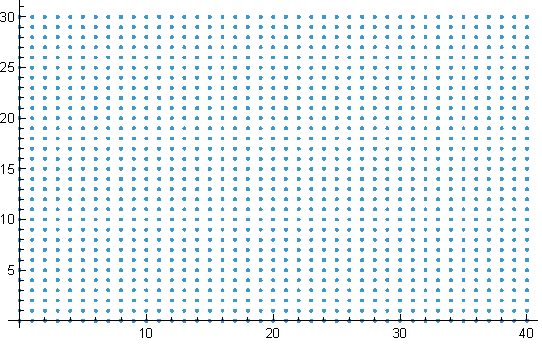
\includegraphics[width=0.5\textwidth]{Stadium_Rect.pdf}
    \caption{Estadio rectángular con $L_x = 40,\, L_y=30$}
\end{figure}
\begin{itemize}
    \item DoS:
    \begin{figure}[H]
    \centering
    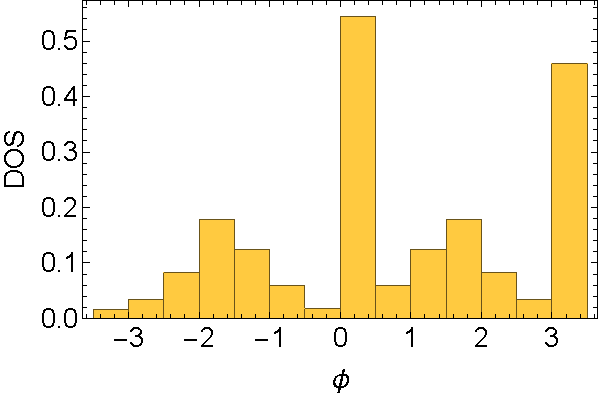
\includegraphics[width=0.6\textwidth]{DoS_Rect_Grover.pdf}
    \caption{DoS, notar las degeneraciones para $0$ y $\pi$}
\end{figure}
    \item $P(s)$:
    \begin{figure}[H]
    \centering
    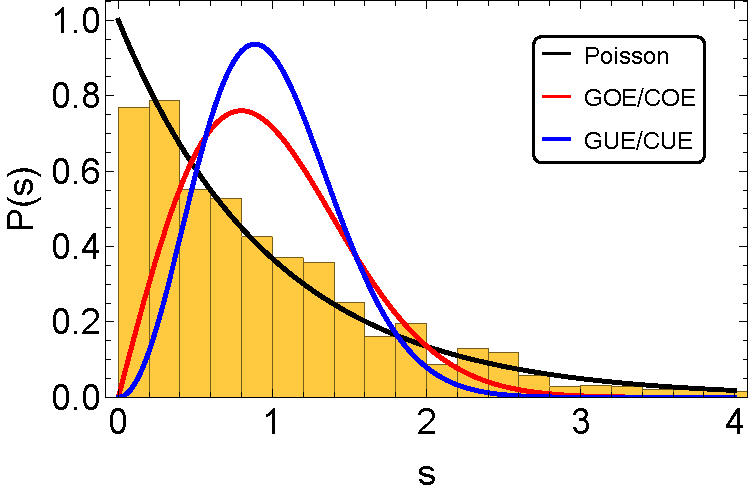
\includegraphics[width=0.6\textwidth]{Ps_Rect_Grover.pdf}
    \caption{$P(s)$, para este cálculo se excluyeron los valores degenerados de $0$ y $\pi$}
\end{figure}
\newpage
    \item $SFF$:
    \begin{figure}[H]
    \centering
    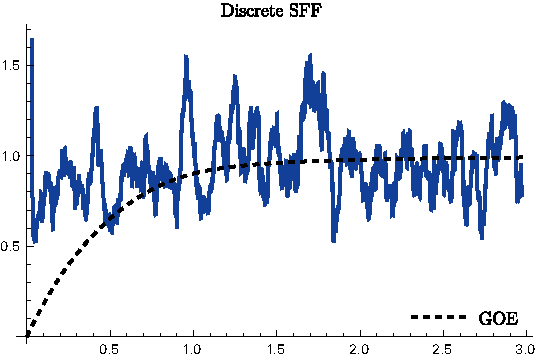
\includegraphics[width=0.6\textwidth]{SFF_Rect_Grover.pdf}
    \caption{$SFF$, para este cálculo se excluyeron los valores degenerados de $0$ y $\pi$}
\end{figure}
\end{itemize}

\subsubsection{Para un estadio triangular:}
Empleando un estadio triangular de lado $L=49$.
\begin{figure}[H]
    \centering
    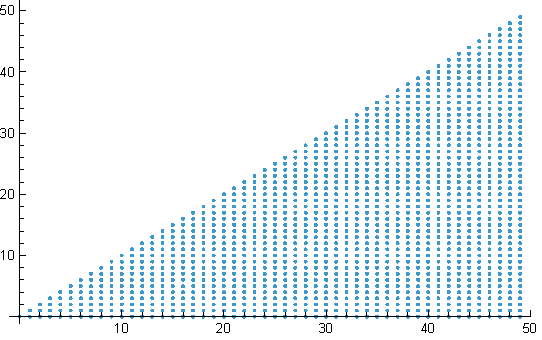
\includegraphics[width=0.5\textwidth]{Stadium_Triangle.pdf}
    \caption{Estadio rectángular con $L_x = 40,\, L_y=30$}
\end{figure}
\begin{itemize}
    \newpage
    \item DoS:
    \begin{figure}[H]
    \centering
    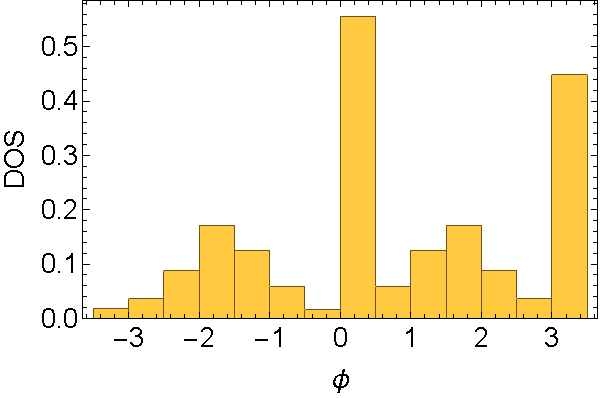
\includegraphics[width=0.6\textwidth]{DoS_Triangle_Grover.pdf}
    \caption{DoS, notar las degeneraciones para $0$ y $\pi$}
\end{figure}
    \item $P(s)$:
    \begin{figure}[H]
    \centering
    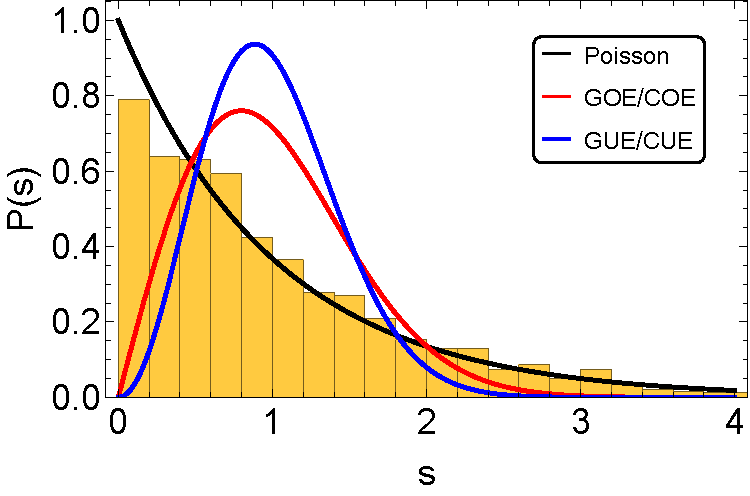
\includegraphics[width=0.6\textwidth]{Ps_Triangle_Grover.pdf}
    \caption{$P(s)$, para este cálculo se excluyeron los valores degenerados de $0$ y $\pi$}
\end{figure}
\newpage
    \item $SFF$:
    \begin{figure}[H]
    \centering
    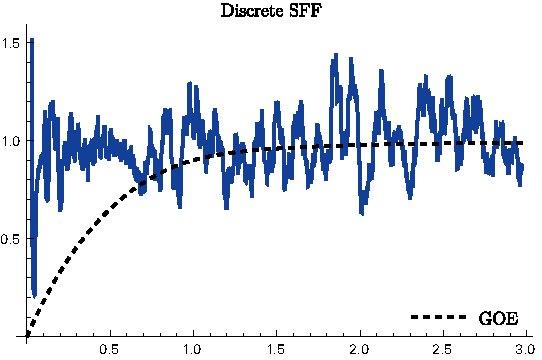
\includegraphics[width=0.6\textwidth]{SFF_Triangle_Grover.pdf}
    \caption{$SFF$, para este cálculo se excluyeron los valores degenerados de $0$ y $\pi$}
\end{figure}
\end{itemize}

\subsubsection{Para un estadio 1/8 de sinaí:}
Empleando un estadio triangular de lado $L=63$ y $R=44$.
\begin{figure}[H]
    \centering
    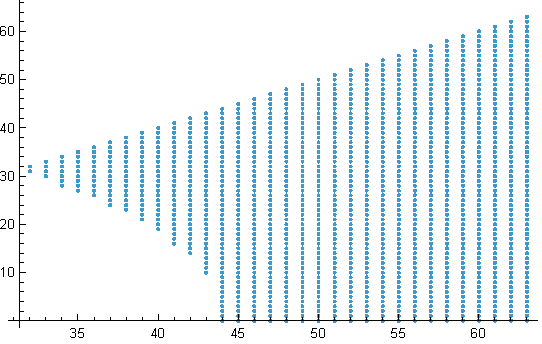
\includegraphics[width=0.5\textwidth]{Stadium_Sinai.pdf}
    \caption{Estadio rectángular con $L_x = 40,\, L_y=30$}
\end{figure}
\begin{itemize}
    \newpage
    \item DoS:
    \begin{figure}[H]
    \centering
    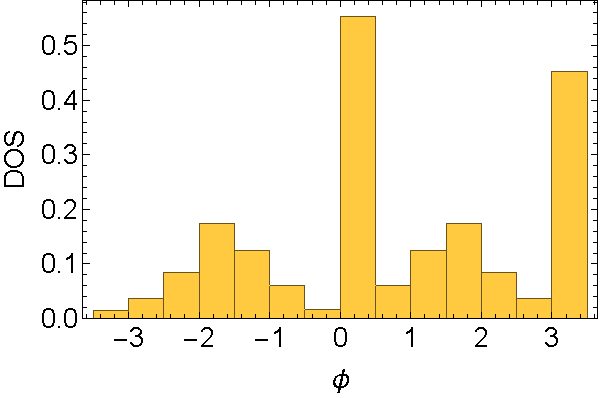
\includegraphics[width=0.6\textwidth]{DoS_Sinai_Grover.pdf}
    \caption{DoS, notar las degeneraciones para $0$ y $\pi$}
\end{figure}
    \item $P(s)$:
    \begin{figure}[H]
    \centering
    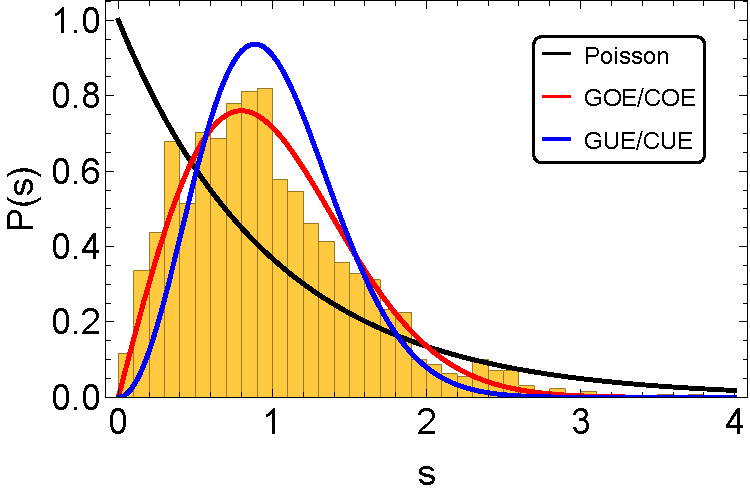
\includegraphics[width=0.6\textwidth]{Ps_Sinai_Grover.pdf}
    \caption{$P(s)$, para este cálculo se excluyeron los valores degenerados de $0$ y $\pi$}
\end{figure}
\newpage
    \item $SFF$:
    \begin{figure}[H]
    \centering
    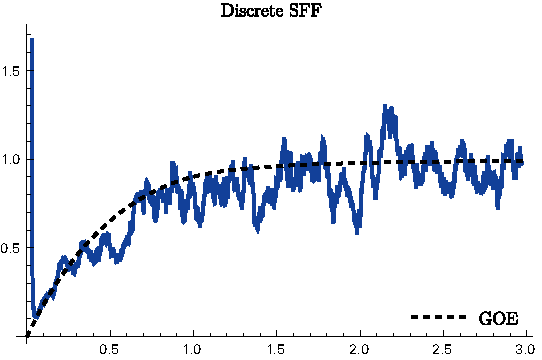
\includegraphics[width=0.6\textwidth]{SFF_Sinai_Grover.pdf}
    \caption{$SFF$, para este cálculo se excluyeron los valores degenerados de $0$ y $\pi$}
\end{figure}
\end{itemize}

% *}}}
\subsection{Dinámica según una moneda de Haadamar:} % {{{*
\subsubsection{Para un estadio rectangular}
Empleando un estadio rectángular con $L_x = 40,\, L_y=30$.
\begin{figure}[H]
    \centering
    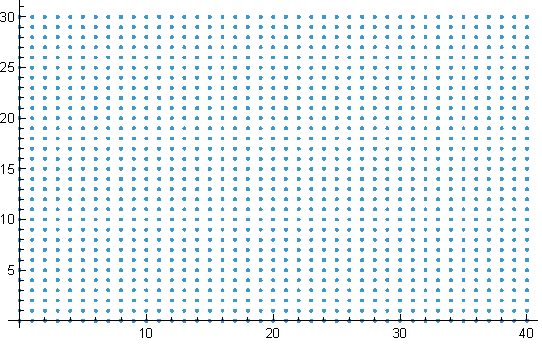
\includegraphics[width=0.5\textwidth]{Stadium_Rect.pdf}
    \caption{Estadio rectángular con $L_x = 40,\, L_y=30$}
\end{figure}
\begin{itemize}
    \item DoS:
    \begin{figure}[H]
    \centering
    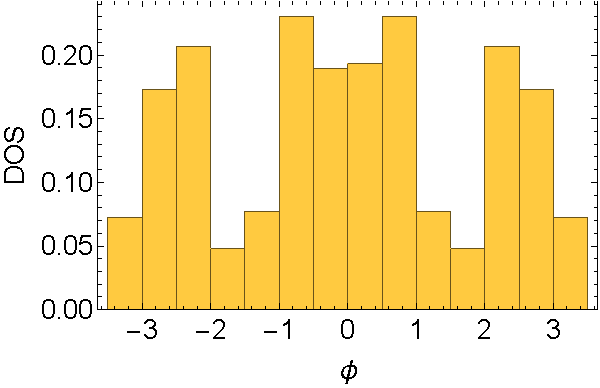
\includegraphics[width=0.6\textwidth]{DoS_Rect_Haad.pdf}
    \caption{DoS.}
\end{figure}
    \item $P(s)$:
    \begin{figure}[H]
    \centering
    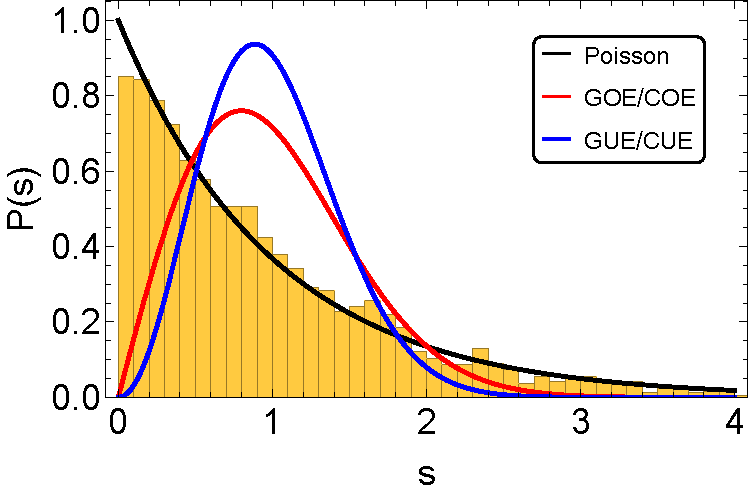
\includegraphics[width=0.6\textwidth]{Ps_Rect_Haad.pdf}
    \caption{$P(s)$.}
\end{figure}
\newpage
    \item $SFF$:
    \begin{figure}[H]
    \centering
    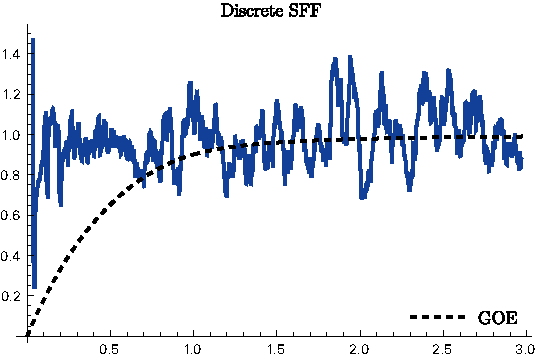
\includegraphics[width=0.6\textwidth]{SFF_Rect_Haad.pdf}
    \caption{$SFF$.}
\end{figure}
\end{itemize}

\subsubsection{Para un estadio triangular:}
Empleando un estadio triangular de lado $L=49$.
\begin{figure}[H]
    \centering
    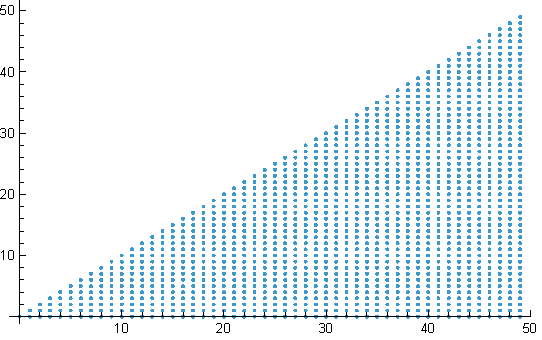
\includegraphics[width=0.5\textwidth]{Stadium_Triangle.pdf}
    \caption{Estadio rectángular con $L_x = 40,\, L_y=30$}
\end{figure}
\begin{itemize}
    \newpage
    \item DoS:
    \begin{figure}[H]
    \centering
    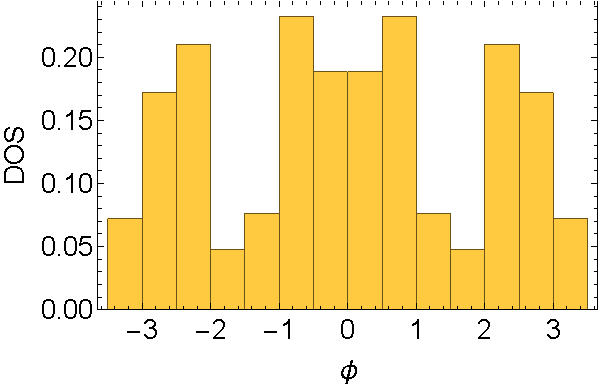
\includegraphics[width=0.6\textwidth]{DoS_Triangle_Haad.pdf}
    \caption{DoS.}
\end{figure}
    \item $P(s)$:
    \begin{figure}[H]
    \centering
    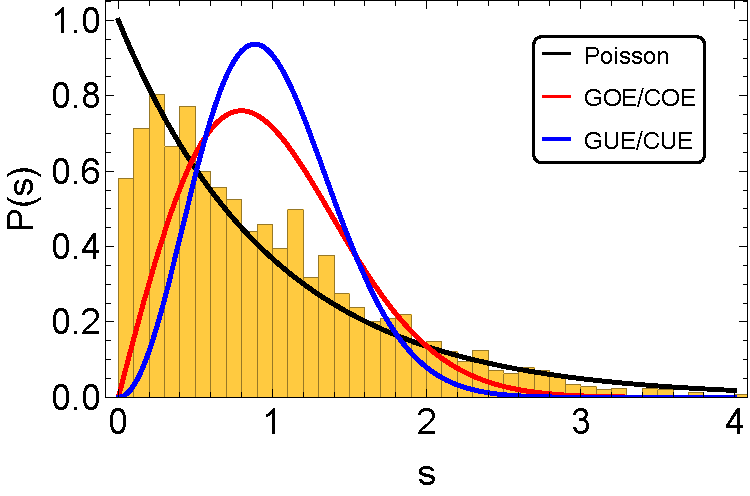
\includegraphics[width=0.6\textwidth]{Ps_Triangle_Haad.pdf}
    \caption{$P(s)$.}
\end{figure}
\newpage
    \item $SFF$:
    \begin{figure}[H]
    \centering
    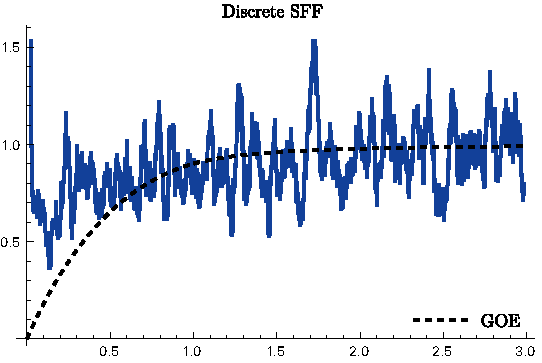
\includegraphics[width=0.6\textwidth]{SFF_Triangle_Haad.pdf}
    \caption{$SFF$.}
\end{figure}
\end{itemize}

\subsubsection{Para un estadio 1/8 de sinaí:}
Empleando un estadio triangular de lado $L=63$ y $R=44$.
\begin{figure}[H]
    \centering
    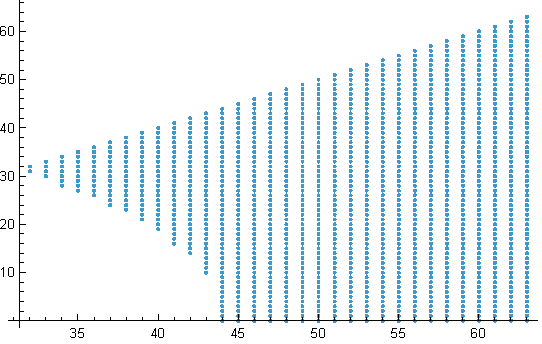
\includegraphics[width=0.5\textwidth]{Stadium_Sinai.pdf}
    \caption{Estadio rectángular con $L_x = 40,\, L_y=30$}
\end{figure}
\begin{itemize}
    \newpage
    \item DoS:
    \begin{figure}[H]
    \centering
    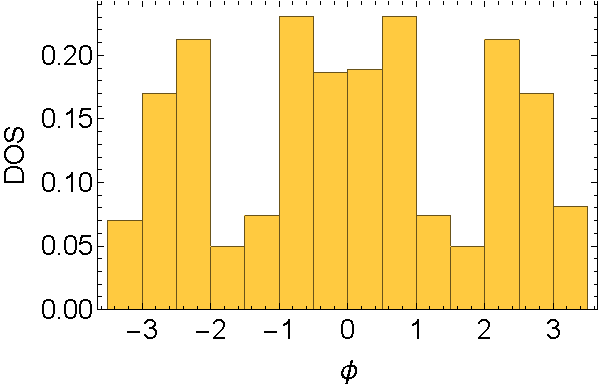
\includegraphics[width=0.6\textwidth]{DoS_Sinai_Haad.pdf}
    \caption{DoS.}
\end{figure}
    \item $P(s)$:
    \begin{figure}[H]
    \centering
    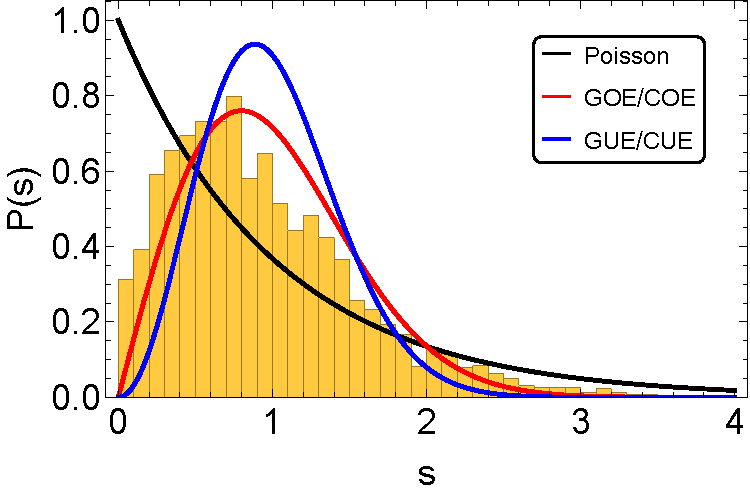
\includegraphics[width=0.6\textwidth]{Ps_Sinai_Haad.pdf}
    \caption{$P(s)$.}
\end{figure}
\newpage
    \item $SFF$:
    \begin{figure}[H]
    \centering
    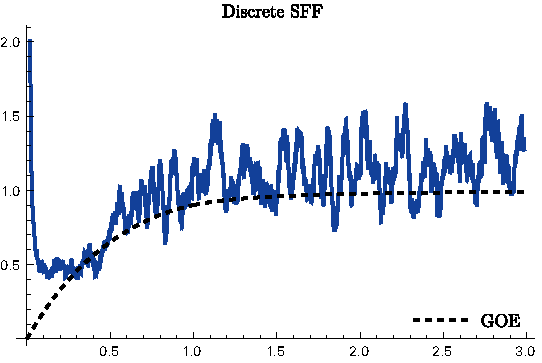
\includegraphics[width=0.6\textwidth]{SFF_Sinai_Haad.pdf}
    \caption{$SFF$.}
\end{figure}
\end{itemize}

% *}}}
\subsection{Dinámica según una moneda aleatoria del ensamble COE:} % {{{*
La moneda pertenece a una muestra del ensamble circular ortogonal.
\subsubsection{Para un estadio rectangular}
Empleando un estadio rectángular con $L_x = 40,\, L_y=30$.
\begin{figure}[H]
    \centering
    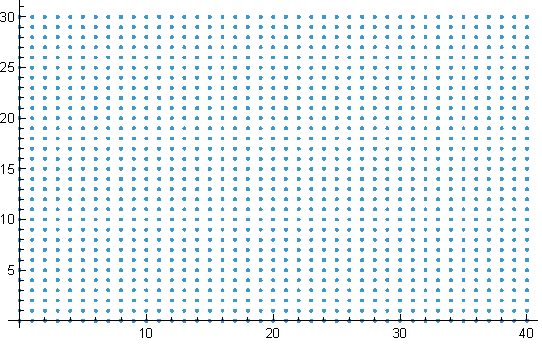
\includegraphics[width=0.5\textwidth]{Stadium_Rect.pdf}
    \caption{Estadio rectángular con $L_x = 40,\, L_y=30$}
\end{figure}
\begin{itemize}
    \item DoS:
    \begin{figure}[H]
    \centering
    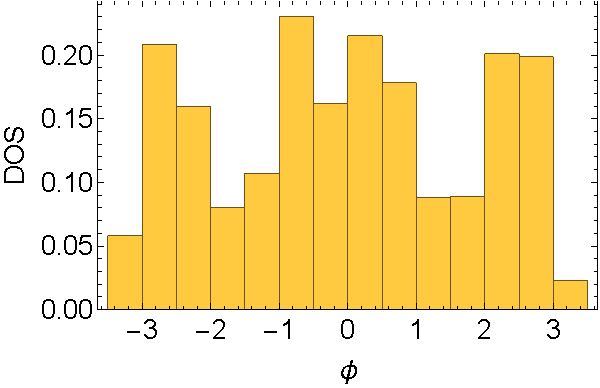
\includegraphics[width=0.6\textwidth]{DoS_Rect_RndCOE.pdf}
    \caption{DoS.}
\end{figure}
    \item $P(s)$:
    \begin{figure}[H]
    \centering
    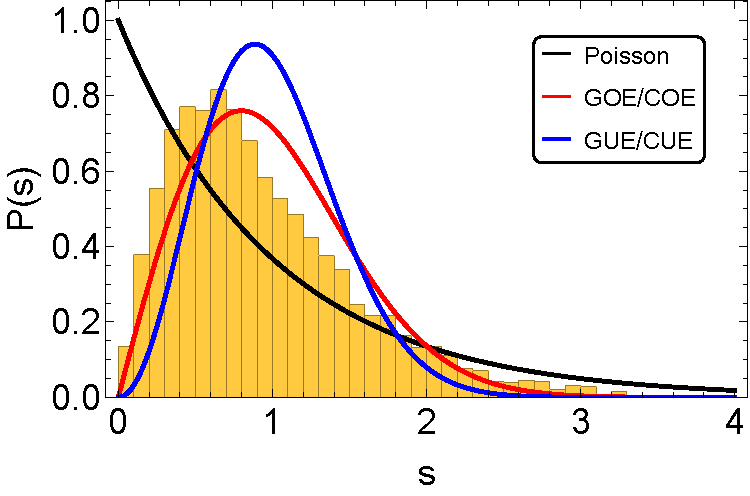
\includegraphics[width=0.6\textwidth]{Ps_Rect_RndCOE.pdf}
    \caption{$P(s)$.}
\end{figure}
\newpage
    \item $SFF$:
    \begin{figure}[H]
    \centering
    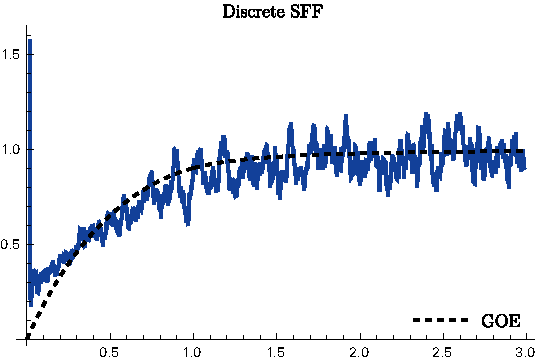
\includegraphics[width=0.6\textwidth]{SFF_Rect_RndCOE.pdf}
    \caption{$SFF$.}
\end{figure}
\end{itemize}

\subsubsection{Para un estadio triangular:}
Empleando un estadio triangular de lado $L=49$.
\begin{figure}[H]
    \centering
    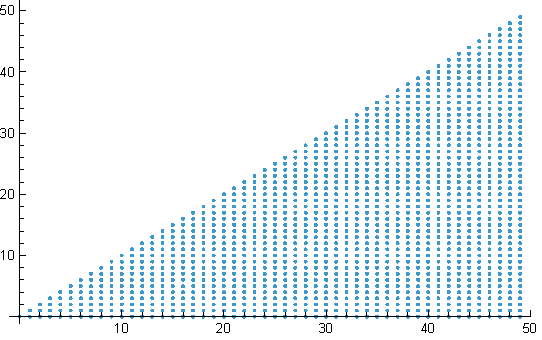
\includegraphics[width=0.5\textwidth]{Stadium_Triangle.pdf}
    \caption{Estadio rectángular con $L_x = 40,\, L_y=30$}
\end{figure}
\begin{itemize}
    \newpage
    \item DoS:
    \begin{figure}[H]
    \centering
    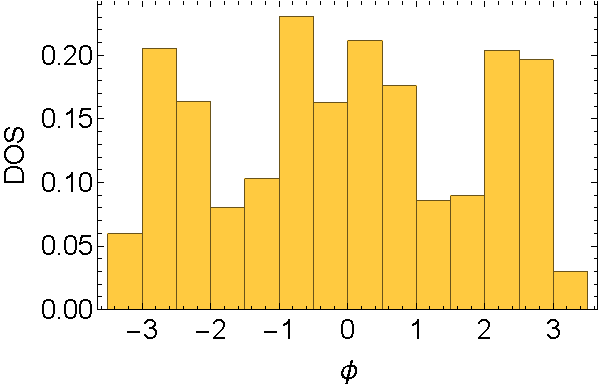
\includegraphics[width=0.6\textwidth]{DoS_Sinai_RndCOE.pdf}
    \caption{DoS.}
\end{figure}
    \item $P(s)$:
    \begin{figure}[H]
    \centering
    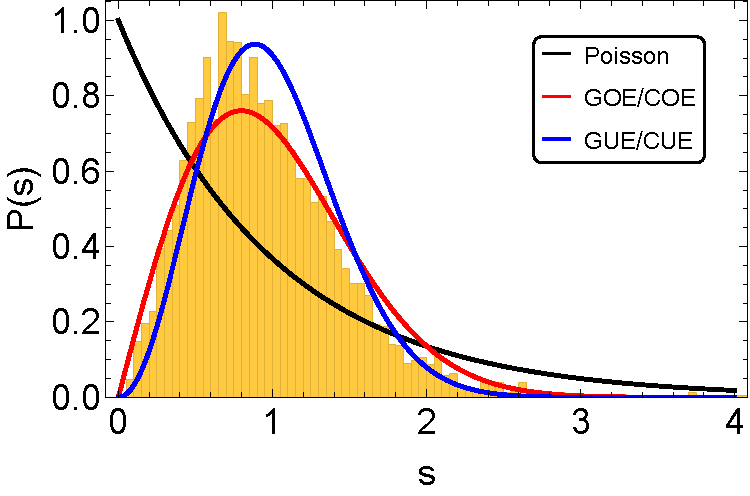
\includegraphics[width=0.6\textwidth]{Ps_Triangle_RndCOE.pdf}
    \caption{$P(s)$.}
\end{figure}
\newpage
    \item $SFF$:
    \begin{figure}[H]
    \centering
    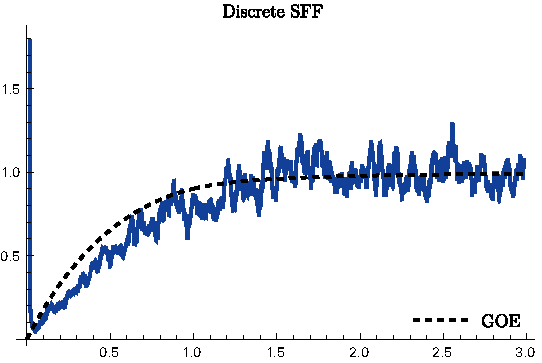
\includegraphics[width=0.6\textwidth]{SFF_Triangle_RndCOE.pdf}
    \caption{$SFF$.}
\end{figure}
\end{itemize}

\subsubsection{Para un estadio 1/8 de sinaí:}
Empleando un estadio triangular de lado $L=63$ y $R=44$.
\begin{figure}[H]
    \centering
    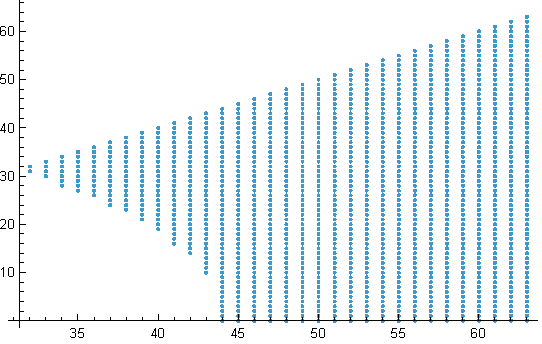
\includegraphics[width=0.5\textwidth]{Stadium_Sinai.pdf}
    \caption{Estadio rectángular con $L_x = 40,\, L_y=30$}
\end{figure}
\begin{itemize}
    \newpage
    \item DoS:
    \begin{figure}[H]
    \centering
    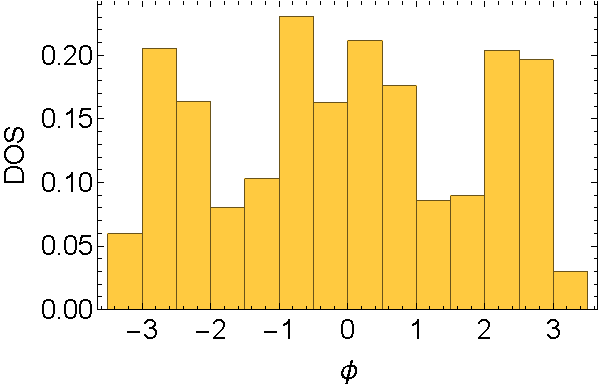
\includegraphics[width=0.6\textwidth]{DoS_Sinai_RndCOE.pdf}
    \caption{DoS.}
\end{figure}
    \item $P(s)$:
    \begin{figure}[H]
    \centering
    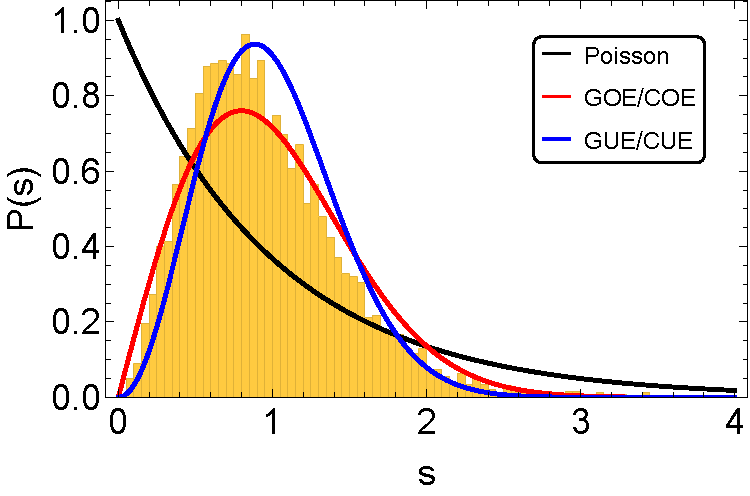
\includegraphics[width=0.6\textwidth]{Ps_Sinai_RndCOE.pdf}
    \caption{$P(s)$.}
\end{figure}
\newpage
    \item $SFF$:
    \begin{figure}[H]
    \centering
    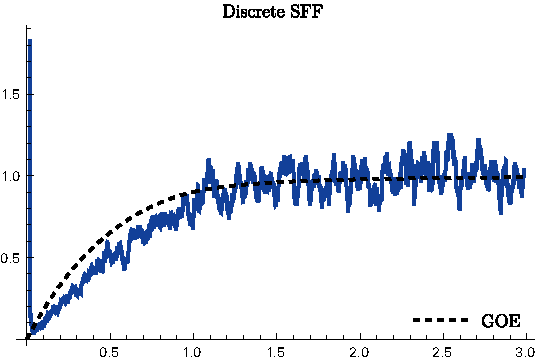
\includegraphics[width=0.6\textwidth]{SFF_Sinai_RndCOE.pdf}
    \caption{$SFF$.}
\end{figure}
\end{itemize}
% *}}}

% --- NUEVA SECCIÓN DE BIBLIOGRAFÍA ---
\bibliographystyle{plain}
\bibliography{ref}

\end{document}